% Sơ đồ kiến trúc giải thích contract; không đo latency hoặc causal effect.
\documentclass[10pt]{article}
\usepackage[T1]{fontenc}
\usepackage{lmodern}
\usepackage[paperwidth=180mm,paperheight=150mm,margin=4mm]{geometry}
\usepackage{tikz}
\usetikzlibrary{arrows.meta,positioning}
\pagestyle{empty}
\setlength{\parindent}{0pt}
\hyphenpenalty=10000
\exhyphenpenalty=10000
\definecolor{ink}{HTML}{1F3445}
\definecolor{teal}{HTML}{126B80}
\definecolor{violet}{HTML}{6D548A}
\definecolor{ochre}{HTML}{9A581D}
\begin{document}
\centering
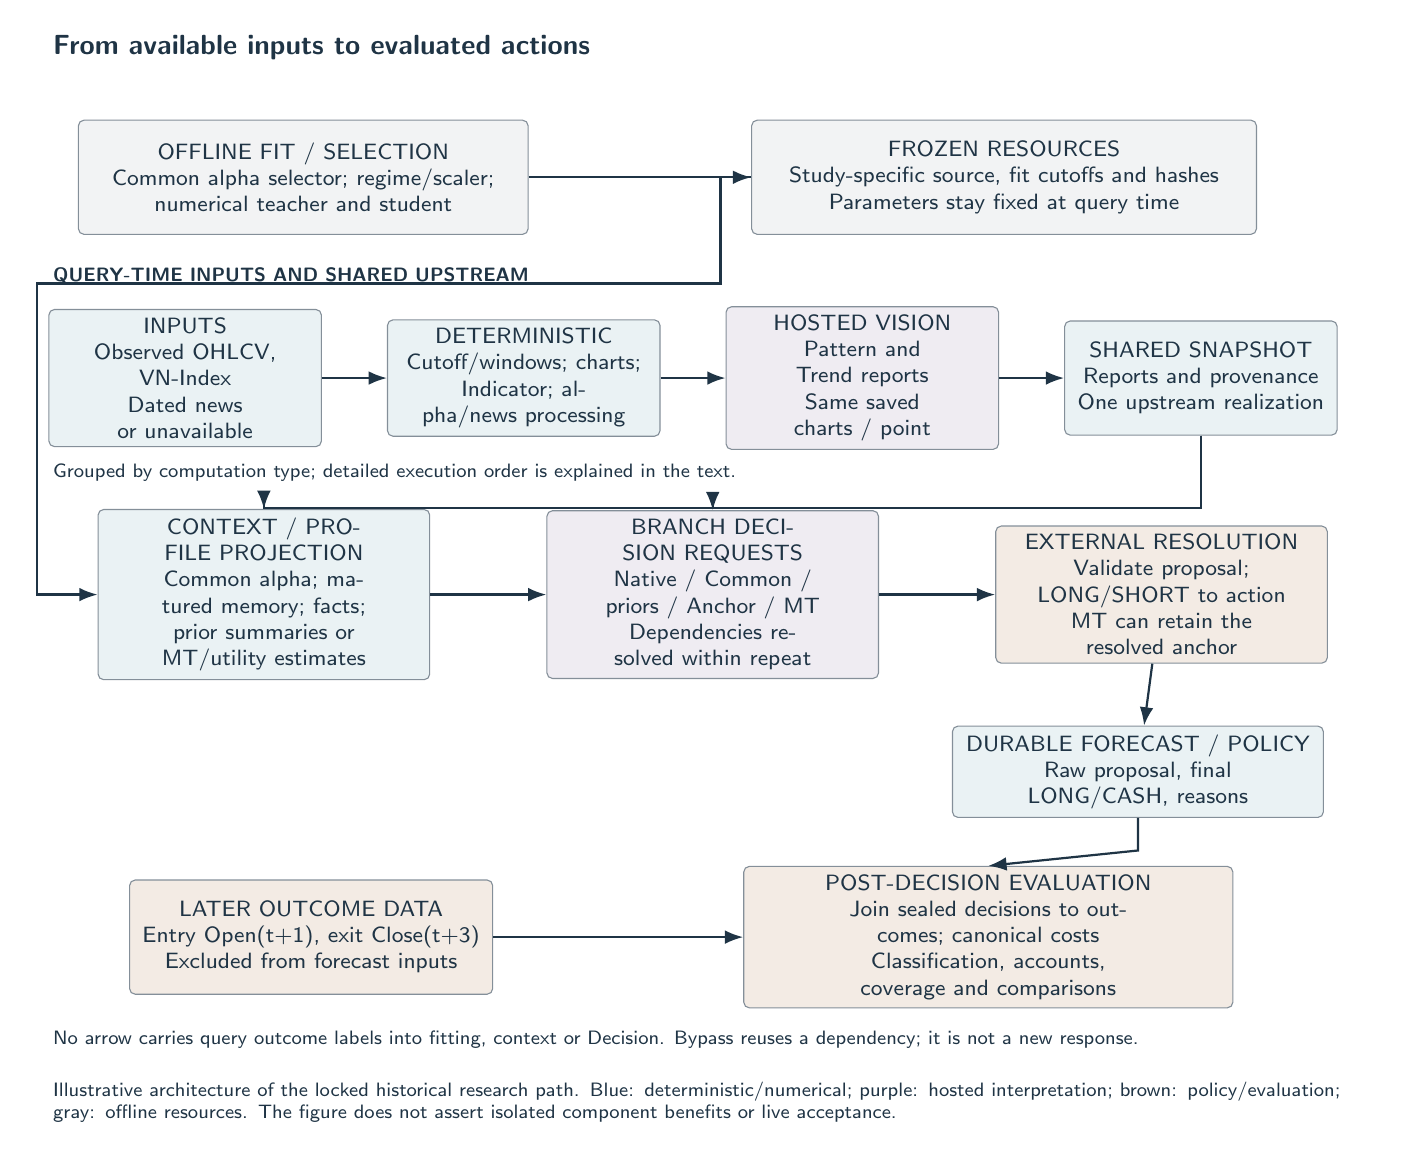
\begin{tikzpicture}[x=1cm,y=1cm,>=Latex,font=\sffamily\footnotesize,text=ink,
 box/.style={draw=ink!55,rounded corners=2pt,align=center,text width=3.25cm,minimum height=1.45cm,inner sep=3pt},
 flow/.style={->,thick,draw=ink}]
\path[use as bounding box] (0,0) rectangle (17.1,14.1);
\node[anchor=west,font=\sffamily\bfseries] at (.2,13.85) {From available inputs to evaluated actions};
\node[box,fill=ink!6,text width=5.5cm] (fit) at (3.5,12.2)
 {OFFLINE FIT / SELECTION\\Common alpha selector; regime/scaler;\\numerical teacher and student};
\node[box,fill=ink!6,text width=6.2cm] (res) at (12.4,12.2)
 {FROZEN RESOURCES\\Study-specific source, fit cutoffs and hashes\\Parameters stay fixed at query time};
\draw[flow] (fit) -- (res);
\node[anchor=west,font=\sffamily\bfseries\scriptsize] at (.2,10.95) {QUERY-TIME INPUTS AND SHARED UPSTREAM};
\node[box,fill=teal!9] (data) at (2.0,9.65)
 {INPUTS\\Observed OHLCV, VN-Index\\Dated news or unavailable};
\node[box,fill=teal!9] (prep) at (6.3,9.65)
 {DETERMINISTIC\\Cutoff/windows; charts;\\Indicator; alpha/news processing};
\node[box,fill=violet!11] (vision) at (10.6,9.65)
 {HOSTED VISION\\Pattern and Trend reports\\Same saved charts / point};
\node[box,fill=teal!9] (shared) at (14.9,9.65)
 {SHARED SNAPSHOT\\Reports and provenance\\One upstream realization};
\draw[flow] (data) -- (prep);
\draw[flow] (prep) -- (vision);
\draw[flow] (vision) -- (shared);
\node[anchor=west,font=\sffamily\scriptsize] at (.2,8.45)
 {Grouped by computation type; detailed execution order is explained in the text.};
\node[box,fill=teal!9,text width=4.0cm] (context) at (3.0,6.9)
 {CONTEXT / PROFILE PROJECTION\\Common alpha; matured memory; facts;\\prior summaries or MT/utility estimates};
\node[box,fill=violet!11,text width=4.0cm] (decision) at (8.7,6.9)
 {BRANCH DECISION REQUESTS\\Native / Common / priors / Anchor / MT\\Dependencies resolved within repeat};
\node[box,fill=ochre!12,text width=4.0cm] (policy) at (14.4,6.9)
 {EXTERNAL RESOLUTION\\Validate proposal; LONG/SHORT to action\\MT can retain the resolved anchor};
\draw[flow] (context) -- (decision);
\draw[flow] (decision) -- (policy);
\draw[flow] (shared.south) -- (14.9,8.0) -- (8.7,8.0) -- (decision.north);
\draw[flow] (shared.south) -- (14.9,8.0) -- (3.0,8.0) -- (context.north);
\draw[flow] (res.west) -- (8.8,12.2) -- (8.8,10.85) -- (.12,10.85) -- (.12,6.9) -- (context.west);
\node[box,fill=teal!9,text width=4.5cm,minimum height=1.0cm] (durable) at (14.1,4.65)
 {DURABLE FORECAST / POLICY\\Raw proposal, final LONG/CASH, reasons};
\draw[flow] (policy) -- (durable);
\node[box,fill=ochre!12,text width=4.4cm] (outcome) at (3.6,2.55)
 {LATER OUTCOME DATA\\Entry Open(t+1), exit Close(t+3)\\Excluded from forecast inputs};
\node[box,fill=ochre!12,text width=6.0cm] (evaluation) at (12.2,2.55)
 {POST-DECISION EVALUATION\\Join sealed decisions to outcomes; canonical costs\\Classification, accounts, coverage and comparisons};
\draw[flow] (outcome) -- (evaluation);
\draw[flow] (durable.south) -- (14.1,3.65) -- (evaluation.north);
\node[anchor=west,font=\sffamily\scriptsize] at (.2,1.25)
 {No arrow carries query outcome labels into fitting, context or Decision. Bypass reuses a dependency; it is not a new response.};
\node[anchor=west,align=left,text width=16.7cm,font=\sffamily\scriptsize] at (.2,.45)
 {Illustrative architecture of the locked historical research path. Blue: deterministic/numerical; purple: hosted interpretation;
 brown: policy/evaluation; gray: offline resources. The figure does not assert isolated component benefits or live acceptance.};
\end{tikzpicture}
\end{document}
